\section{Introduction}

Convolutional neural networks (CNNs) are often used for image segmentation tasks. However, pixel-wise accuracy does not guarantee that the predicted segmentation preserves correct structural properties. This shortcoming is evident in conventional and more sophisticated loss functions such as generalized Dice loss\supercite{Sudre:2017}. Furthermore, a large dataset is not always a practical or sufficient solution, especially in fields such as medical imaging, where data annotation can be expensive. This motivates the development of a topological loss function\supercite{Clough:2022}, which is the subject of this replication. \\

The main condition that the topological loss function requires is that the underlying topology of the images can be specified in advance. Then, there are two frameworks for applying the loss function, namely post-processing and semi-supervised frameworks. The idea of both frameworks is to combine some standard loss function to train the model with a topological loss function that incrementally updates the established model weights (during or after training) to penalize any violations of the specified underlying structure. \\

In this replication, we implement two out of four experiments of the paper from scratch as no publicly available code is supplemented by the authors\footnote{In the paper, the authors provide a sample repository for the first (MNIST) experiment\supercite{Repo_mnist}. However, the code does not fully follow the specified process of training the CNNs as described in the paper.}. We attempt to verify the usefulness of a topological loss function in image segmentation tasks and provide a more thorough description of how the frameworks can be implemented in practice.

\section{Replication Scope}

As mentioned in the introduction, we only implement two out of four experiments conducted in the original paper due to data availability issues. In particular, data for Experiment 2 requires approval from UK Biobank\supercite{UK_Biobank}, whereas data for Experiment 4 was not released due to lack of patient consent\supercite{Clough:2022}. \\

Since the semi-supervised framework was only applied to Experiment 2, we evaluate the post-processing framework exclusively.
Our primary objective is to verify whether the numerical claims made by the authors can be reproduced, which consists of two parts. First, we investigate whether the post-processing framework improves segmentation performance. Second, we assess whether our models achieve results comparable with the paper.

\section{Topological Loss Implementation}

In this section, we discuss the theory behind the topological loss function and the post-processing framework. Then, we establish an algorithmic implementation of the framework.

\subsection{Topological Priors}

To properly define a topological loss function, we have to begin by making our data compatible with topological data analysis tools. For this purpose, we use a cubical complex, which is a collection of points, unit lines, squares, and other higher-dimensional structures (it is similar to a simplicial complex but more appropriate for 2D images and 3D volumes). Since the replicated experiments only used 2D images, we restrict the discussion to this dimension. \\

Define an image represented as a 2D array $X$ with pixel intensities $X_{ij}$. Define the segmentation of some object as a 2D array $S$, but instead of using pixel intensities, let $S_{ij} \in [0,1]$ represent the predicted probability that the pixel belongs to the segmented object. In this paper, $S$ will always be a prediction of some CNN. Then, we consider super-level sets $B$ of $S$ which are defined as collections of pixels for which $S_{ij} \geq p$ for some threshold probability $p$. In particular,
\[
B(p) := \bigcup_{i,j \colon \ S_{ij} \geq p} [i, i+1]\times[j, j+1].
\]
Then, $B(p)$ is a cubical complex with the property that $B(p_1) \subseteq B(p_2)$ whenever $p_1 \geq p_2$. \\

Next, we apply persistent homology by tracking the changes in topological features as we explore all different values of $p\in[0,1]$. In particular, we will track the number of connected components $\beta_0$ and the number of loops $\beta_1$. As a result, we get a set of birth and death values for each topological feature. We will use the same notation as the paper, denoting the birth of the $l$-th longest bar of dimension $k$ by $b_{k,l}$ and death by $d_{k,l}$. For the remainder of the paper, we will consider the variable $t=1-p$ instead, where we start at $t=0$ and end at $t=1$ such that birth values come before death values. Naturally, the bigger the difference $d_{k,l} - b_{k,l}$, the more persistent the feature is. A common way to display all birth and death values is by using a barcode diagram. This process is illustrated in Figure \ref{fig:mnist_cubical_barcode}. Finally, the calculation of births/deaths in such a way is differentiable almost everywhere with respect to the predicted pixel probabilities\supercite{Clough:2022}, and thus also with respect to the neural network's weights, which allows us to update them.

\begin{figure}[H]
    \centering
    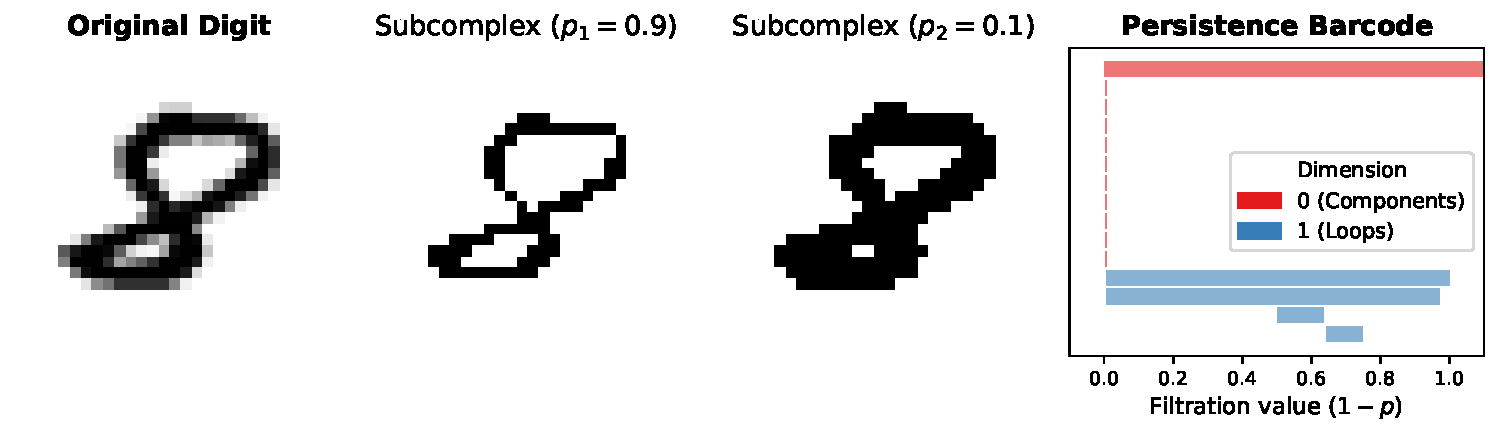
\includegraphics[width=\linewidth]{mnist_cubical_barcode.pdf}
    \caption{From left to right: the original grayscale image, the cubical subcomplexes evaluated at thresholds $p_1 = 0.9$ and $p_2 = 0.1$, and the persistence barcode. The barcode tracks feature lifespans along the filtration parameter $t = 1 - p \in [0, 1]$, highlighting one essential connected component ($\beta_0 = 1$) and two prominent, long-lived loops ($\beta_1 = 2$) corresponding to the two holes of the digit, while short bars reflect short-lived boundary noise.}
    \label{fig:mnist_cubical_barcode}
\end{figure}


\subsection{Topological Loss Function}

We start by specifying the desired structure of the segmented object by $\beta^*_k$ (called the target Betti number at dimension $k$). For the experiments, we will use the fact that $\beta^*_0$ corresponds to the number of connected components and $\beta^*_1$ corresponds to the number of holes/loops, and will denote the specified structure by $H$. For example, $\beta^*_0=1$ means that there is one connected component, $\beta^*_1=0$ means that there are no loops, and $H=(\beta^*_0=1, \beta^*_1=0)$. \\

The loss function for a barcode diagram can be defined as
\[
\mathcal{L}_k(\beta^*_k) = \sum_{l=1}^{\beta^*_k}(1 - |d_{k,l} - b_{k,l}|^2) + \sum_{l=\beta^*_k + 1}^{\infty}|d_{k,l} - b_{k,l}|^2,
\]
\[
\mathcal{L}_\text{topo} = \sum_{k} \mathcal{L}_k(\beta^*_k).
\]
Intuitively, $\mathcal{L}_k(\beta^*_k)$ is minimized when $\beta^*_k$ longest bars are fully persistent bars (i.e. $b_{k,l}=0$, $d_{k,l}=1$) and all other bars have zero length. \\

Following the original paper, we compute persistence barcodes and gradients using the \texttt{TopologyLayer} library\supercite{Gabrielsson:2020}, which introduces three practical adjustments to $\mathcal{L}_k(\beta_k^*)$. First, we drop the constant $1$ since its gradient is zero. Second, we truncate the infinite sum at the $K_{\max} = 15$ longest bars per dimension, minimizing
\[
-\sum_{l=1}^{\beta_k^*} |d_{k,l} - b_{k,l}|^2 + \sum_{l=\beta_k^*+1}^{15} |d_{k,l} - b_{k,l}|^2.
\]
Third, \texttt{TopologyLayer} omits the infinite-persistence $0$-dimensional bar that always exists on a 2D grid and only returns finite bars. To account for this missing component, we set the target bar count for $k=0$ to $\tilde{\beta}_0^* = \max(0, \beta_0^* - 1)$. Consequently, $\beta_0^* = 0$ (an empty image) and $\beta_0^* = 1$ (one component) both yield $\tilde{\beta}_0^* = 0$ and optimize the exact same objective, which is a limitation of the library.


\subsection{Post-Processing Framework}

For the post-processing framework, we begin by training a CNN in a supervised manner, using a regular loss function, to achieve a set of weights $w$. Then, for each item $X_n$ in the test set, we make a copy of weights $w_n=w$ and run gradient descent with respect to $w_n$ on the loss function defined by
\[
\mathcal{L}(X_n; w, w_n) = \frac{1}{V}\|f(X_n,w) - f(X_n,w_n)\|^2 + \lambda \mathcal{L}_\text{topo}(X_n, w_n).
\]
Here, $V$ is the number of pixels in the image and $f(X_n, \cdot)$ is a CNN prediction using weights $\cdot$. The $\|f(X_n,w) - f(X_n,w_n)\|^2$ term acts as a regularizer whereas the $\lambda \mathcal{L}_\text{topo}$ term fixes the topological mistakes in the segmentation. We summarize this process in Algorithm~\ref{alg:topo_post_processing}. Note that for each sample we update a copy of weights $w_n$ while maintaining original weights $w$ fixed.  \\

\begin{algorithm}[H]
\caption{Topological Post-Processing Framework}
\label{alg:topo_post_processing}
\begin{algorithmic}[1]
\Require Pre-trained weights $w$, test sample $X_n$, target Betti numbers $H_n$, regularization weight $\lambda$, learning rate $\eta$, iterations $N_\text{iter}$.
\Ensure Post-processed segmentation prediction $f(X_n, w_n)$.
\State $w_n \gets w$ \Comment{Initialize sample-specific weights}
\For{$t = 1$ \textbf{to} $N_\text{iter}$}
    \State Compute regularizer: $\mathcal{L}_{\text{reg}} \gets \frac{1}{V} \|f(X_n, w) - f(X_n, w_n)\|^2$
    \State Compute topological loss: $\mathcal{L}_{\text{topo}} \gets \mathcal{L}_{\text{topo}}(f(X_n, w_n); H_n)$
    \State Evaluate total loss: $\mathcal{L} \gets \mathcal{L}_{\text{reg}} + \lambda \mathcal{L}_{\text{topo}}$
    \State Update $w_n$ using Adam with learning rate $\eta$ and gradient $\nabla_{w_n}\mathcal{L}$
\EndFor
\State \textbf{return} $f(X_n, w_n)$
\end{algorithmic}
\end{algorithm}


\section{Experiment 1}

In the first experiment, the authors used the MNIST dataset to assess the effects on de-noising quality when applying a topological loss. Denote original digits by $Y$ and corrupted images by $X$, where the corruption is done via a Fourier transform, removing $m$ vertical and $m$ horizontal lines. The idea of the experiment is to train a U-net CNN\supercite{Ronneberger:2015} on a small sample of $(X_\text{train}, Y_\text{train})$ pairs by minimizing MSE. Then, we test de-noising quality on a larger $(X_\text{test}, Y_\text{test})$ sample and assess whether further applying the post-processing framework improves it.

\subsection{Outlined Process}

We start by highlighting all the details mentioned in the original paper. The CNN was trained with $N_\text{train}=100$ samples using a specified U-net architecture. Then, $N_\text{test}=1000$ samples were used to test the reconstruction quality before and after applying the post-processing framework. The quality of de-noising was assessed in two ways: by computing MSE of the predicted and ground-truth images and by computing the classification accuracy of another CNN on the reconstructed images. For classification, a CNN was trained on $N_\text{train}=10000$ separate digits. This experiment was repeated six times, using different noise levels $m\in \{ 2,4,6,8,10,12 \}$. \\

Finally, for the post-processing framework, the authors reported using the lambda value of $\lambda=0.02$. The specified desired Betti numbers were:
\begin{itemize}
  \item $\beta^*_0 = 1, \beta^*_1 = 0$ for numbers $1, 2, 3, 4, 5, 7$;
  \item $\beta^*_0 = 1, \beta^*_1 = 1$ for numbers $0, 6, 9$;
  \item $\beta^*_0 = 1, \beta^*_1 = 2$ for number $8$.
\end{itemize}
Recall that $\beta^*_0$ corresponds to connected components and is therefore always $1$ if an object exists in the image; $\beta^*_1$ corresponds to loops/holes and is therefore varied across different digits. Finally, the number $2$ has two representations in the MNIST dataset, one with a loop and one without. Since the authors marked all digits $2$ with $\beta^*_1 = 0$, we use the same convention for consistency. \\

\subsection{Our Implementation}

We started our replication by \textbf{loading the dataset}. The MNIST dataset was fetched from \texttt{torchvision.datasets.MNIST} and rescaled using min-max scaling. For image corruption, we followed the process described by the authors and used min-max renormalization for the outputs. \\

We proceeded by training the \textbf{classifier model}. The classifier was adapted from the authors' sample repository\supercite{Repo_mnist} and consists of nine convolutional layers followed by three fully connected layers and a final output layer with ten units. All convolutional layers use $3\times3$ kernels and ReLU activations. The third and sixth convolutional layers use a stride of $2$, reducing the spatial dimensions of the input from $28\times28$ to $14\times14$ and then to $7\times7$, while increasing the number of filters from $16$ to $32$ and then $64$. The resulting feature map is flattened and passed through three fully connected layers with $64$ units each before the final classification layer. To train the model, we used the following parameters:
\begin{itemize}
  \item $N_\text{train}=10000$ digits (specified by the authors);
  \item Batch size of $64$;
  \item $250$ epochs;
  \item Adam optimizer with $\eta=10^{-3}$;
  \item Cross-entropy loss.
\end{itemize}
The parameters were selected experimentally based on model performance and without formal hyper-tuning. Finally, for evaluation we use $N_\text{test}=10000$ digits. On uncorrupted digits, our classifier achieved a score of $98.8\%$, which closely matches the authors' reported accuracy of $98.7\%$. \\

We continued by iterating through all noise levels $m$. During each loop, we first trained the \textbf{ main segmenter model}. The CNN uses a U-net-like architecture as described by the authors with two downsampling and two upsampling stages. The encoder consists of convolutional blocks with $16$, $32$, and $64$ filters, respectively, with the first two blocks containing two convolutional layers and the final block containing three. Each convolution is followed by batch normalization and ReLU activation. The decoder uses skip connections from the corresponding encoder blocks and consists of two convolutional blocks with $32$ and $16$ filters. Finally, a $1\times1$ convolution followed by a sigmoid activation produces the reconstructed image. To train the model, we used the following parameters:
\begin{itemize}
  \item $N_\text{train}=100$ digits (specified by the authors);
  \item Batch size of $100$;
  \item $1000$ epochs;
  \item Adam optimizer with $\eta=10^{-3}$;
  \item MSE loss (specified by the authors).
\end{itemize}
We used a high number of epochs to ensure that further optimization primarily reflects the post-processing procedure rather than simply continued training. \\

Finally, we applied the \textbf{post-processing framework}. We used the specified value of $\lambda=0.02$. However, the learning rate and number of iterations for the algorithm were not reported in the original paper. Thus, we conducted a grid search across two noise levels ($m=4, 10$) using a validation set of $N_{\text{val}}=250$ samples. We evaluated learning rates $\eta \in \{ 10^{-3}, 10^{-4}, 10^{-5} \}$ and iteration counts $N_\text{iter} \in \{ 20, 50, 80 \}$, recording both reconstruction MSE and classification accuracy. We found that for this experiment, the hyperparameter sensitivity was quite low. In particular, MSE varied by at most $0.002$ and accuracy by $2$ percentage points. Therefore, we selected a balanced combination of parameters, namely $\eta = 10^{-4}$ and $N_\text{iter} = 50$. Detailed grid search results are presented in Appendix A.

\subsection{Computational Requirements}

The replication was performed using one L4 GPU. The full experiment takes around $100$ minutes to run, while the grid search requires an additional $70$ minutes.

\subsection{Results}

\begin{table}[H]
\centering
\resizebox{\linewidth}{!}{%
\begin{tabular}{r cccc cccc}
\toprule
& \multicolumn{4}{c}{\textbf{Classification Accuracy (\%)}} & \multicolumn{4}{c}{\textbf{Mean Squared Error (MSE)}} \\
\cmidrule(lr){2-5} \cmidrule(lr){6-9}
& \multicolumn{2}{c}{Original Paper} & \multicolumn{2}{c}{Replication (Ours)} & \multicolumn{2}{c}{Original Paper} & \multicolumn{2}{c}{Replication (Ours)} \\
\cmidrule(lr){2-3} \cmidrule(lr){4-5} \cmidrule(lr){6-7} \cmidrule(lr){8-9}
$m$ & $\mathcal{L}_{\text{MSE}}$ & $\mathcal{L}_{\text{topo}}$ & $\mathcal{L}_{\text{MSE}}$ & $\mathcal{L}_{\text{topo}}$ & $\mathcal{L}_{\text{MSE}}$ & $\mathcal{L}_{\text{topo}}$ & $\mathcal{L}_{\text{MSE}}$ & $\mathcal{L}_{\text{topo}}$ \\
\midrule
2  & 95.7 & 96.2     & 97.2 & 98.0$^*$ & 0.008 & 0.008 & 0.005 & 0.006$^*$ \\
4  & 92.9 & 93.7     & 94.0 & 95.1$^*$ & 0.014 & 0.013 & 0.012 & 0.011$^*$ \\
6  & 87.6 & 90.8$^*$ & 89.0 & 90.8$^*$ & 0.023 & 0.023 & 0.019 & 0.018$^*$ \\
8  & 80.4 & 86.0$^*$ & 81.2 & 84.6$^*$ & 0.037 & 0.028 & 0.027 & 0.027$^*$ \\
10 & 70.4 & 75.0$^*$ & 71.0 & 73.5$^*$ & 0.032 & 0.033 & 0.038 & 0.038\phantom{$^*$} \\
12 & 56.9 & 63.0$^*$ & 51.4 & 54.4$^*$ & 0.043 & 0.042 & 0.053 & 0.054$^*$ \\
\bottomrule
\end{tabular}%
}
\caption{Replication of Experiment 1 results across noise levels $m$, comparing baseline ($\mathcal{L}_{\text{MSE}}$) and post-processed ($\mathcal{L}_{\text{topo}}$) models against Clough et al. Asterisks ($^*$) indicate statistical significance at $p < 0.05$ (McNemar's test for accuracy; two-sided Wilcoxon signed-rank test for MSE).}
\label{tab:mnist_results}
\end{table}

Table \ref{tab:mnist_results} presents our replicated findings alongside the results reported by the authors. Our replicated accuracy values closely match the original paper across all noise levels, with the only meaningful deviation at $m=12$. While the authors found statistically significant accuracy improvements for higher noise ($m \ge 6$), our replication yielded statistically significant improvements across all tested noise levels. \\

Furthermore, both studies suggest that topological post-processing has a limited effect on pixel-wise MSE. The authors reported no statistically significant MSE changes ($p > 0.05$). In contrast, our two-sided Wilcoxon signed-rank tests detected statistically significant differences at several noise levels. However, the absolute differences were small, amounting to a change of at most $0.001$ based on the rounded values in Table~\ref{tab:mnist_results}. In particular, MSE is higher after post-processing for $m=2,12$, lower for $m=4,6,8$ and insignificant for $m=10$. \\


We also note a possible typographical error in the original paper's Table 1. The reported baseline MSE increases to $0.037$ at $m=8$ before decreasing to $0.032$ at $m=10$, contrary to the overall trend of increasing reconstruction error with noise. The possibly correct value of $0.027$ would restore this trend and match our replicated baseline MSE at $m=8$. However, without access to the authors' underlying results, we cannot establish whether the reported value is erroneous.


\section{Experiment 3}

In the third experiment, the authors used the Automated Cardiac Diagnosis Challenge (ACDC) dataset\supercite{Bernard:2018} to test whether the post-processing framework achieves comparable performance to other segmentation models. The dataset consists of $150$ complete 3D MRI volumes ($100$ train, $50$ test) across healthy and unhealthy patients, where one set of scans consists of a patient's end-diastole (heart fully relaxed) and end-systole (heart fully squeezed). The authors began by training a U-net CNN\supercite{Ronneberger:2015} to segment the myocardium of the left ventricle (which looks like a donut when the volume is sliced), and then applied the post-processing framework. The final results were evaluated with mean Dice score of end-diastole and end-systole separately.


\subsection{Outlined Process}

The authors trained their CNN on the full $N_\text{train}=100$ patients ($1902$ 2D slices) using binary cross-entropy. Then, they manually labeled $N_\text{test}=50$ patients' images ($1076$ 2D slices) for their underlying topology. The three outlined scenarios for an image were:
\begin{itemize}
    \item $\beta^*_0 = 0, \beta^*_1 = 0$ when no myocardium is present;
    \item $\beta^*_0 = 1, \beta^*_1 = 0$ when we see a solid block of a myocardium with no hole (vertex of the left ventricle);
    \item $\beta^*_0 = 1, \beta^*_1 = 1$ when myocardium is present in a donut-shape.
\end{itemize}
Finally, the authors report using the lambda value of $\lambda=0.01$ and Dice score for their final results.


\subsection{Our Implementation}

We began the replication by \textbf{loading the dataset}. The dataset was downloaded from a public online repository via \texttt{huggingface\_hub}. We used a custom-written class to convert 3D volumes to a 2D data structure that is compatible with \texttt{PyTorch}. We clipped pixel values below the 1st and above the 99th percentiles to avoid extreme MRI intensity artifacts, standardized each slice using $z$-score normalization, and spatially interpolated all slices and masks to $256 \times 256$ pixels (using bilinear and nearest-neighbor interpolation, respectively). \\

We proceeded by training our \textbf{main segmenter model}. No architecture was described by the authors, so we used a 4-level (or depth-3) U-net architecture which is common for image segmentation tasks \supercite{Ronneberger:2015} \supercite{Bernard:2018}. In particular, the architecture consists of three downsampling and three upsampling stages. The encoder consists of four convolutional blocks with $32$, $64$, $128$, and $256$ filters, respectively, with each block containing two convolutional layers followed by batch normalization and ReLU activation. The decoder uses skip connections from the corresponding encoder blocks and consists of three convolutional blocks with $128$, $64$, and $32$ filters. A final $1\times1$ convolution followed by a sigmoid activation produces the segmentation output. \\

An addition to the training process was the use of early stopping, which was mentioned by the authors in Experiment 2. For this purpose, we used roughly a quarter of test data ($256$/$1076$ images). Overall, the following parameters were used:
\begin{itemize}
    \item $N_\text{train}=100$ patients (specified by the authors);
    \item Batch size of $32$;
    \item $200$ epochs;
    \item Adam optimizer with $\eta=10^{-3}$ and a weight decay of $10^{-5}$;
    \item Cosine Annealing with $\eta_\text{min} = 10^{-6}$ across all epochs;
    \item Binary cross-entropy loss (specified by the authors);
    \item Early-stopping patience level of $15$ epochs (activated after epoch $50$ based on validation Dice score).
\end{itemize}
The hyper-parameters were once again selected experimentally to achieve model performance that was close to the authors' final results. \\

For the \textbf{post-processing framework}, we used the specified lambda value of $\lambda = 0.01$. Since the public repository included ground-truth segmentation masks for the test set, we extracted the target Betti numbers in-code rather than labeling all $1076$ slices manually, as the authors originally did. Specifically, we applied connected-component labeling to each binary myocardium mask to count connected components and to its inverted background (excluding the outer boundary) to count enclosed holes. As with Experiment 1, we still needed to hyper-tune the learning rate and number of iterations of the framework. For this, we used $\eta\in\{10^{-5}, 10^{-6}, 10^{-7} \}, N_\text{iter} \in \{5, 10, 20 \}$ and a subset of the test set with $N_\text{val} = 256$ images. We found that $\eta=10^{-5}$ and $N_\text{iter}=5$ performed the best across both end-diastole and end-systole (for full results see Appendix A). \\

Finally, for evaluation, we used continuous 2D slice predictions which were thresholded at $0.5$ and stacked to compute 3D segmentation volumes. Then, we computed the volumetric Dice similarity coefficient for each patient volume at end-diastole (ED) and end-systole (ES).


\subsection{Computational Requirements}

The replication was performed using one L4 GPU. The full experiment takes around $2.5$ hours to run, while the grid search requires an additional $10$ hours using full image resolution. The grid search runs in around $2$ hours if images are rescaled from $256 \times 256$ to $128 \times 128$ pixels without meaningful changes in results.


\subsection{Results}

Before post-processing, our model scored $87.28\%$ on end-diastole and $87.93\%$ on end-systole segmentation using the full test set. After the post-processing framework, the model achieved the scores of $87.69\%$ and $88.23\%$ for end-diastole and end-systole respectively. This marks a marginal improvement of $0.41$ percentage points for end-diastole and $0.30$ percentage points for end-systole using Dice scores. \\

In contrast, the authors report achieving the scores of $89.94\%$ and $90.68\%$ for end-diastole and end-systole. Although the reported figures are higher, there is no evidence about the model performance before the post-processing framework in the paper. This makes our findings difficult to compare, as higher scores could simply be a result of a better-tuned CNN. \\

Finally, due to the limited training set size, we used a subset of the test set for early stopping and hyperparameter tuning, introducing a risk of data leakage. This is a limitation of our implementation, as model selection was not fully independent of the final evaluation data. Consequently, the reported test performance should be interpreted with this limitation in mind.


\section{Discussion and Conclusion}

Overall, the primary claims of the original paper were partially replicated. For Experiment 1, the authors claimed that reconstructed digit classification accuracy was positively affected by the post-processing framework for higher noise levels ($m \geq 6$). While our numerical values differed slightly, we confirmed that a statistically significant improvement in classification accuracy was present at all noise levels, which is an even stronger finding than originally reported. Furthermore, while the authors observed no significant differences in reconstruction MSE before and after topological regularization, we identified a statistically significant difference. As discussed, this effect is small in absolute magnitude and has an inconsistent trend across noise values. \\

For Experiment 3, the authors reported state-of-the-art Dice scores using the framework. Because no baseline was provided to evaluate CNN performance prior to post-processing, we were unable to isolate the exact relative contribution of the framework to that claim. Nonetheless, we observed an overall Dice score improvement of $0.41$ percentage points for end-diastole and $0.30$ percentage points for end-systole after applying the framework. This suggests that even on well-trained models, optimizing a topological loss function can be a viable strategy for refining anatomical predictions, albeit the extent of improvement may be somewhat limited. \\

The primary contribution of this work is providing an open-source, reproducible codebase for the topological post-processing framework. We also provide a pipeline to incorporate this framework into a modern deep learning pipeline, including hyperparameter tuning for learning rates and loss iterations. Finally, we establish baseline comparisons that contextualize the original paper's findings alongside our replicated results.

